\documentclass{article}
\usepackage[UTF8]{ctex}
\usepackage[utf8]{inputenc}
\usepackage{amsmath}
\usepackage{algorithm}  
\usepackage{algcompatible}
\usepackage{algorithmicx}  
\usepackage{algpseudocode}  
\usepackage{listings}
\usepackage{xcolor}
\usepackage{graphicx}
\usepackage{enumerate}

\usepackage{enumitem}
\title{计算机网络实验报告}
\author{作者 }
\date{班级}


\usepackage{listings} 
\usepackage{xcolor}
\lstset{
  language=Matlab,  %代码语言使用的是matlab
  frame=shadowbox, %把代码用带有阴影的框圈起来
  rulesepcolor=\color{red!20!green!20!blue!20},%代码块边框为淡青色
  keywordstyle=\color{blue!90}\bfseries, %代码关键字的颜色为蓝色,粗体
  commentstyle=\color{red!10!green!70}\textit,    % 设置代码注释的颜色
  showstringspaces=false,%不显示代码字符串中间的空格标记
  numbers=left, % 显示行号
  numberstyle=\tiny,    % 行号字体
  stringstyle=\ttfamily, % 代码字符串的特殊格式
  breaklines=true, %对过长的代码自动换行
  extendedchars=false,  %解决代码跨页时,章节标题,页眉等汉字不显示的问题
  escapebegin=\begin{CJK*},escapeend=\end{CJK*},      % 代码中出现中文必须加上,否则报错
  texcl=true}


\lstset{breaklines}%自动将长的代码行换行排版

\lstset{extendedchars=false}%解决代码跨页时,章节标题,页眉等汉字不显示的问题



\begin{document}

\maketitle

\section{路由器配置实验}
\subsection{实验目的}
掌握路由器的基本知识;
掌握路由器端口的配置;
掌握路由协议的基本配置;
熟悉使用Boson Netsim模拟器。

\subsection{实验内容}
本实验要求自行构建一个网络拓扑,要求包括3个以上路由器(路由器采用串行连接),用于连接两个以太网,每个以太网至少包括1台主机;
完成路由器、主机等设备的配置;使用RIP或OSPF来维护路由器的路由表。 
实验配置完成后,两台主机要能够相互ping通
实验报告要包括网络拓扑、配置以及结果

\subsection{实验原理}
\subsubsection{路由器基本结构}

路由器由存储器、处理器、网络接口等组成;
路由器型号不同,端口数目和类型也不尽相同。

\subsubsection{路由器的接口类型}

网络接口:局域网接口,广域网接口等,其中局域网接口包括以太网接口,快速以太网接口、千兆以太网接口、串口、光纤接口等。
管理接口:控制台接口,辅助接口
\subsubsection{路由器的配置模式}
4种基本模式:\par
用户模式> ,
特权模式 \# 

配置模式(config)\# ,
端口配置模式(config-if)\# ,

\subsubsection{路由器一般步骤}
创建拓扑图:设备:路由器,交换机,主机等。
连接:类型,端口。
\par

配置路由器端口:路由器LAN端口的配置(以太网端口)
或路由器WAN端口的配置(串口serial0,serial1)
\par

路由协议的配置:配置RIP,OSPF
注意:对于路由协议的配置是在路由器端口正确配置的前提下进行的。
\par

路由测试:在PC机或路由器上使用ping命令ping其它路由器以太网端口,从而判断路由协议是否正确。

\subsection{实验过程}
\subsubsection{创建拓扑图}
根据实验要求的网络拓扑结构,选择网络设备,并把这些网络设备连接起来。

\begin{figure}[H]
    \centering
    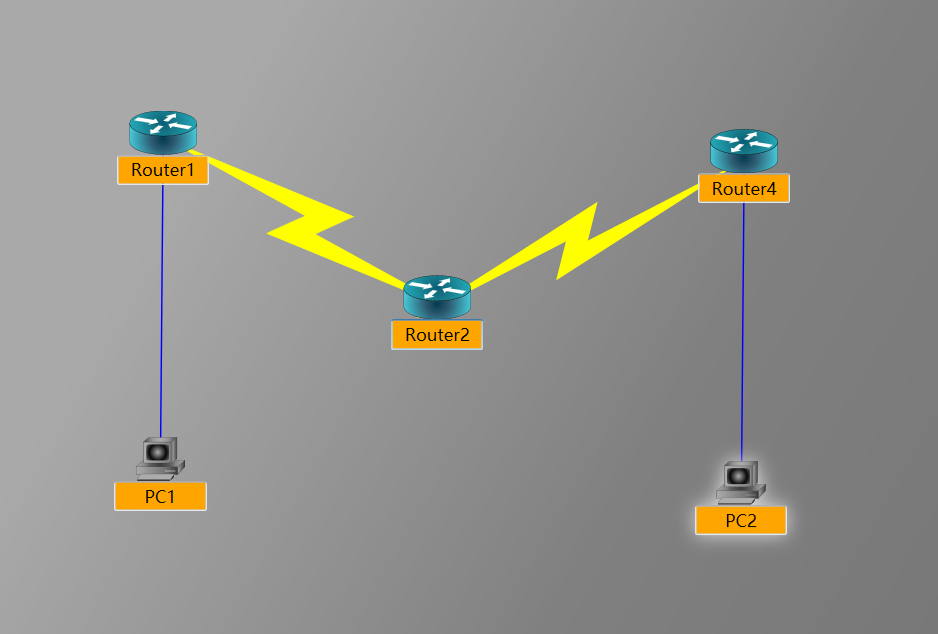
\includegraphics[width=3in]{pic.PNG}
\end{figure} 

\subsubsection{配置路由器}
配置各路由器和PC的接口,为了能够使非直连的网络可以互通,通过手工配置的方法来添加静态路由。\par
本次实验采用RIP方法,端口参数如下:
\begin{table}[]
\begin{tabular}{llllll}
           & PC1         & Router1     & Router2     & Router3     & PC2         \\
Ethernet 0 & 192.168.2.1 & 192.168.1.1 & /           & 192.168.4.1 & 192.168.4.2 \\
Serial 0   & /           & 192.168.2.1 & 192.168.2.2 & 192.168.3.2 & /           \\
Serial 1   & /           & /           & 192.168.3.1 & /           & /          
\end{tabular}
\end{table}

Router1
\begin{lstlisting}
enable
configure terminal
hostname Route1

% connect to PC1
interface ethernet 0
ip address 192.168.1.1 255.255.255.0
no shutdown

% connect to route3
interface serial 0
ip address 192.168.2.1 255.255.255.0
clock rate 64000
no shutdown

ip route 192.168.3.0 255.255.255.0 192.168.2.2
ip route 192.168.4.0 255.255.255.0 192.168.2.2
\end{lstlisting}
Router2
\begin{lstlisting}
enable
configure terminal
hostname Route2
% connect to route1
interface serial 0
ip address 192.168.2.2 255.255.255.0
clock rate 64000
no shutdown

% connect to route3
interface serial 1
ip address 192.168.3.1 255.255.255.0
clock rate 64000
no shutdown

ip route 192.168.1.0 255.255.255.0 192.168.2.1
ip route 192.168.4.0 255.255.255.0 192.168.3.2
\end{lstlisting}

Router3
\begin{lstlisting}
enable
configure terminal
hostname Route3

% connect to route2
interface serial 0
ip address 192.168.3.2 255.255.255.0
clock rate 64000
no shutdown

% connect to PC2
interface ethernet 0
ip address 192.168.4.1 255.255.255.0
no shutdown

ip route 192.168.2.0 255.255.255.0 192.168.3.1
ip route 192.168.1.0 255.255.255.0 192.168.3.1
\end{lstlisting}

\subsubsection{配置PC}
PC1:
\begin{lstlisting}
ipconfig /ip 192.168.1.2 255.255.255.0
ipconfig /dg 192.168.1.1
\end{lstlisting}

PC2:
\begin{lstlisting}
ipconfig /ip 192.168.4.2 255.255.255.0
ipconfig /dg 192.168.4.1
\end{lstlisting}


然后再测试设备之间的连通性。


\subsection{实验结果}
\subsubsection{路由器信息}
通过\emph{show ip route}可以看到,非直连的网络可以互通。
show running-config
\begin{figure}[H]
    \centering
    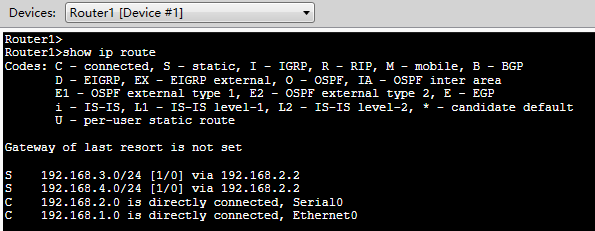
\includegraphics[width=3in]{r1.PNG}
    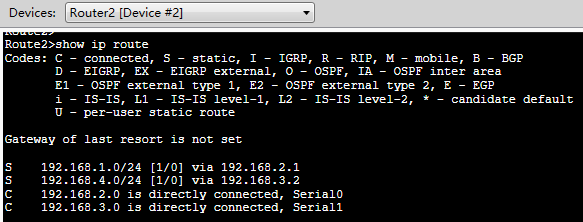
\includegraphics[width=3in]{r2.PNG}
    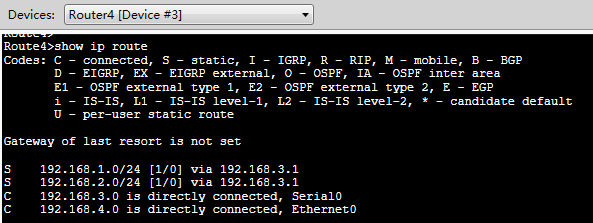
\includegraphics[width=3in]{r3.PNG}
\end{figure} 

\subsubsection{连通情况}
PC1可以ping到PC2;PC2可以ping到PC1;
\begin{figure}[H]
    \centering
    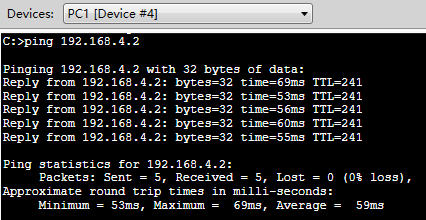
\includegraphics[width=3in]{pc1.PNG}
    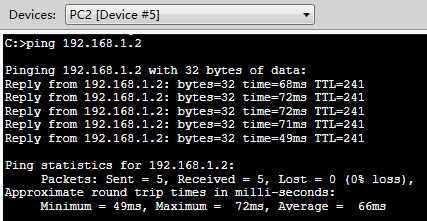
\includegraphics[width=3in]{pc2.PNG}
\end{figure} 
此外,通过\emph{show running-config}也可以观察到,各路由器配置正确。

\newpage

\section{面向HTTP协议的抓包分析实验}


\subsection{实验目的}

\begin{enumerate}[(1)]
    \item 利用Ethereal软件分析HTTP及其下层协议(TCP协议)
    \item 了解网络中数据封装的概念
    \item  掌握HTTP及TCP协议的工作过程。 
\end{enumerate}

\subsection{实验内容}
\begin{enumerate}[(1)]
    \item 启动Ethereal软件,进行报文截获
    \item 在浏览器访问www.xjtu.edu.cn页面。
    \item 分析截获报文。
\end{enumerate}

\subsection{实验原理}
\subsubsection{http协议}

Web的客户/服务器:
略

HTTP服务的特点:

\begin{itemize}
    \item 略
    \item 略
    \item 略
\end{itemize}

\subsubsection{TCP的工作流程}

\begin{enumerate}[(1)]
    \item 三次握手建立连接,略{
    \begin{itemize}
        \item  第一次握手:略
        \item 第二次握手:略
        \item 第三次握手:略
    \end{itemize}
    }
    \item  略
    \item 四次挥手释放连接,略{
    \begin{itemize}
        \item 略
        \item 略
        \item 略
        \item 略
    \end{itemize}
    }
\end{enumerate}


\subsection{实验过程}
\begin{enumerate}[(1)]
    \item 查看www.xjtu.edu.cn对应的ip地址,可以看到其ip地址为202.117.1.13
    \begin{figure}[H]
        \centering
        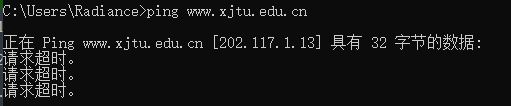
\includegraphics[width=6in]{http0.png}
    \end{figure} 
    \item {打开wireshark软件,在过滤器里利用
    
    \textbf{ip.addr == 202.117.1.13 and (tcp.srcport==<port> or tcp.port==<port>}
    
    过滤出对应数据包}
    \item 从截获的报文中选择HTTP请求报文和HTTP应答报文。
    \begin{figure}[H]
        \centering
        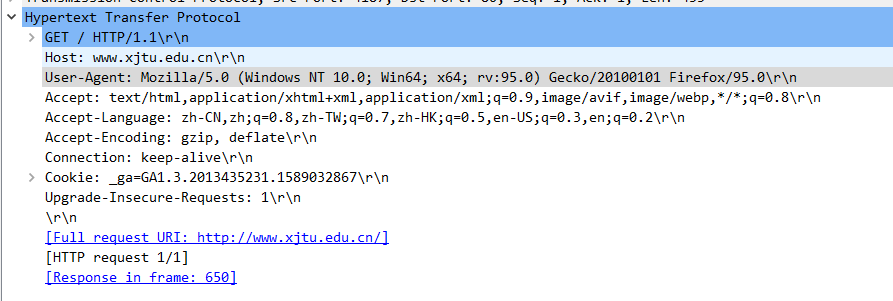
\includegraphics[width=5in]{http2.png}
    \end{figure} 
    HTTP协议的工作过程和各字段的值如2.3.1章节所述。
    
    \item 从截获报文中选择TCP建立连接和释放连接的报文。
    TCP三次握手数据包的序号为518,523,527;挥手数据包的序号为648,649,666。
    \begin{figure}[H]
        \centering
        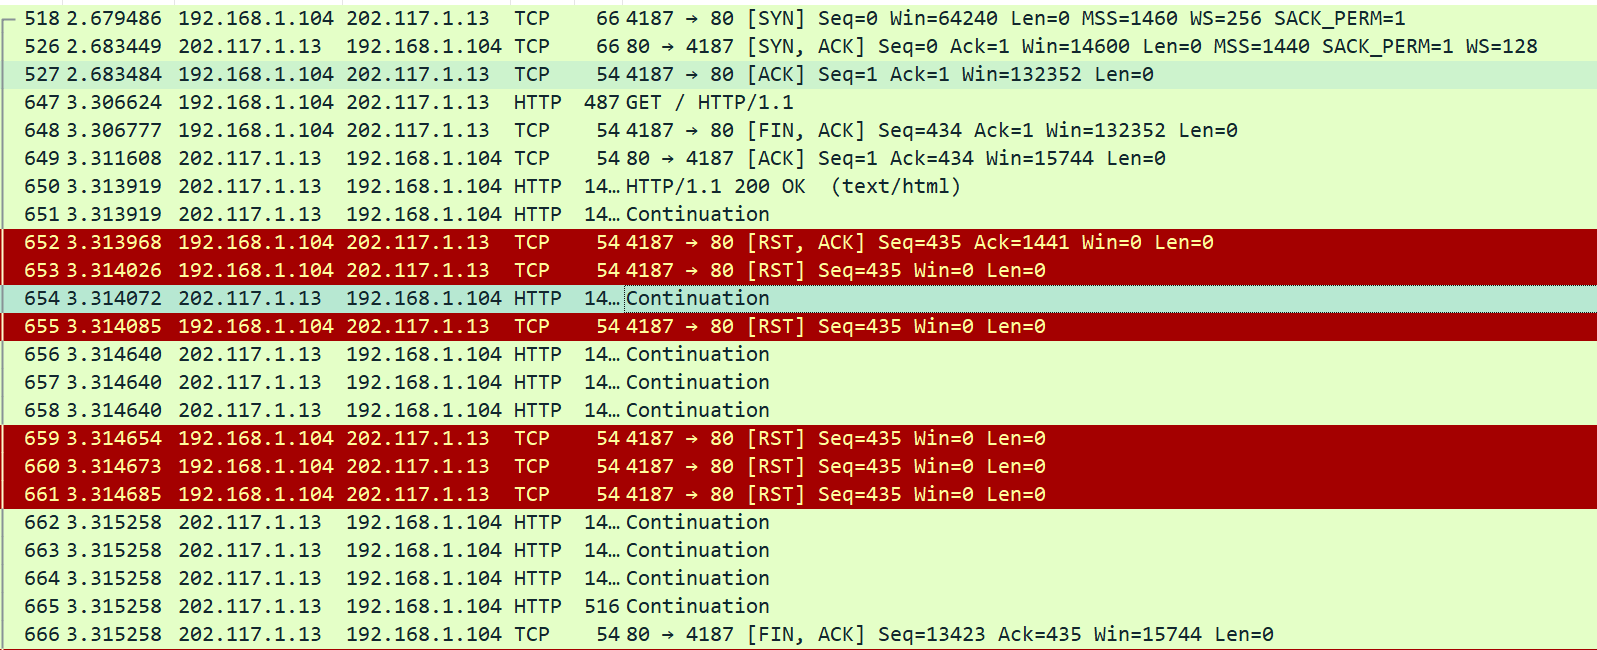
\includegraphics[width=5in]{http1.png}
    \end{figure}
    
    各个字段的值并概括TCP协议的工作过程如2.3.2章节所述。
\end{enumerate}

\subsection{实验总结}
通过wireshark软件抓包,获取了浏览器访问域名服务器时相互交换的TCP与HTTP报文。
了解网络中数据封装的概念,进一步掌握HTTP及TCP协议的工作过程,分析了TCP三次握手、四次挥手的过程。

\end{document}

